\documentclass{exam}

\usepackage{indentfirst}
\usepackage{graphicx}
\usepackage{listings}
\usepackage{color}
\usepackage{fancyvrb}
\usepackage{url}
\usepackage{amsmath}
\usepackage{amssymb}
\usepackage{tikz}
\usepackage{algorithm}
\usepackage{algpseudocode}


\definecolor{mygreen}{rgb}{0,0.6,0}
\definecolor{mygray}{rgb}{0.5,0.5,0.5}
\definecolor{mymauve}{rgb}{0.58,0,0.82}

\lstset{ %
	backgroundcolor=\color{white},		% choose the background color; you must add \usepackage{color} or \usepackage{xcolor}
	basicstyle=\small\ttfamily,		% the size of the fonts that are used for the code
	breakatwhitespace=false,			% sets if automatic breaks should only happen at whitespace
	breaklines=true,					% sets automatic line breaking
	captionpos=b,						% sets the caption-position to bottom
	columns=fullflexible,
	commentstyle=\color{mygreen},		% comment style
	deletekeywords={...},				% if you want to delete keywords from the given language
	escapeinside={\%*}{*)},			% if you want to add LaTeX within your code
	extendedchars=true,				% lets you use non-ASCII characters; for 8-bits encodings only, does not work with UTF-8
	frame=single,						% adds a frame around the code
	keepspaces=true,					% keeps spaces in text, useful for keeping indentation of code (possibly needs columns=flexible)
	keywordstyle=\color{blue},			% keyword style
	language=Octave,					% the language of the code
	morekeywords={*,...},				% if you want to add more keywords to the set
	%   numbers=left,						% where to put the line-numbers; possible values are (none, left, right)
	%   numbersep=6pt,						% how far the line-numbers are from the code
	%   numberstyle=\tiny\color{mygray},	% the style that is used for the line-numbers
	rulecolor=\color{black},			% if not set, the frame-color may be changed on line-breaks within not-black text (e.g. comments (green here))
	showspaces=false,					% show spaces everywhere adding particular underscores; it overrides 'showstringspaces'
	showstringspaces=false,			% underline spaces within strings only
	showtabs=false,					% show tabs within strings adding particular underscores
	stepnumber=1,						% the step between two line-numbers. If it's 1, each line will be numbered
	stringstyle=\color{mymauve},		% string literal style
	tabsize=2,							% sets default tabsize to 2 spaces
	title=\lstname						% show the filename of files included with \lstinputlisting; also try caption instead of title
}

% Creates a new command to include a perl script, the first parameter is the filename of the script (without .pl), the second parameter is the caption
\newcommand{\octavescript}[2]{
	\lstinputlisting[caption=#2]{#1}
}

\newcommand{\MNLab}{Laborator\ \#5}
\newcommand{\MNLabTitle}{Metode iterative pentru rezolvarea sistemelor de ecuații liniare: Jacobi, Gauss-Seidel, Suprarelaxare}
\newcommand{\MNLabTitleHeader}{Metode iterative}
\newcommand{\MNAuthor}{Răgman Andrei, Stan Andrei, Bogdan Țigănoaia}

\renewcommand{\contentsname}{Cuprins}
\renewcommand{\figurename}{Figura}
\renewcommand{\refname}{Referințe}

\setlength{\parskip}{0.5\baselineskip}

\graphicspath{{./img/}}

\title{
	\textmd{\textbf{\MNLabTitle}}
	\author{}
	\date{}
}

\pagestyle{headandfoot}

\header{Metode Numerice}
{\MNLabTitleHeader}
{2025}
\footer{Facultatea de Automatică și Calculatoare}{}{Pagina \thepage\ din \numpages}

\begin{document}

\begin{coverpages}
	\maketitle
	\thispagestyle{empty}
	\tableofcontents
\end{coverpages}

\section{Obiective laborator}

În urma parcurgerii acestui laborator, studentul va fi capabil să rezolve
sisteme de ecuații liniare utilizând metode iterative.

\section{Noțiuni teoretice}

Metodele exacte de rezolvare a sistemelor de ecuații liniare, având complexitate
$O(n^3)$, au aplicabilitate limitată la sisteme de orid relativ mic. Pentru
sisteme de dimensiuni mai mari se utilizează metode iterative, cu complexitate
$O(n^2)$. Acestea utilizează relații de recurență, care prin aplicare repetată
furnizează aproximații, cu precizie controlată, a soluției sistemului.

\subsection{Metode iterative pentru funcții}

Vom dezvolta ideea de \textit{metode iterative} pornind de la un caz mai simplu,
cel al metodelor iterative pentru funcții.

\textbf{Exemplu grafic. Numărul de aur.} Începem cu orice număr real pozitiv $x$
și calculăm
\begin{equation*}
	x^{(k+1)} = \sqrt{1 + x^{(k)}}
\end{equation*}

La un moment dat, $|x^{(k+1)} - x^{(k)}| < \varepsilon$, unde $\varepsilon$ este
o valoare mică dată. Asta înseamnă $x^{(k+1)} \approx x^{(k)}$.
\begin{align*}
	x    & = \sqrt{1 + x}                                     \\
	x^2  & = 1 + x                                            \\
	x^2  & - x - 1 = 0                                        \\
	x    & = \frac{1 \pm \sqrt{5}}{2}                         \\
	\phi & = \frac{1 + \sqrt{5}}{2} \approx 1.618033988749895
\end{align*}

\newpage
Soulția sistemului este dată de intersecția a două funcții: $f(x) = x$ și
$g(x) = \sqrt{1 + x}$. Dacă trasăm grafic aceste puncte, obținem un punct de
intersecție, care este soluția sistemului.

\begin{figure}[h]
	\centering
	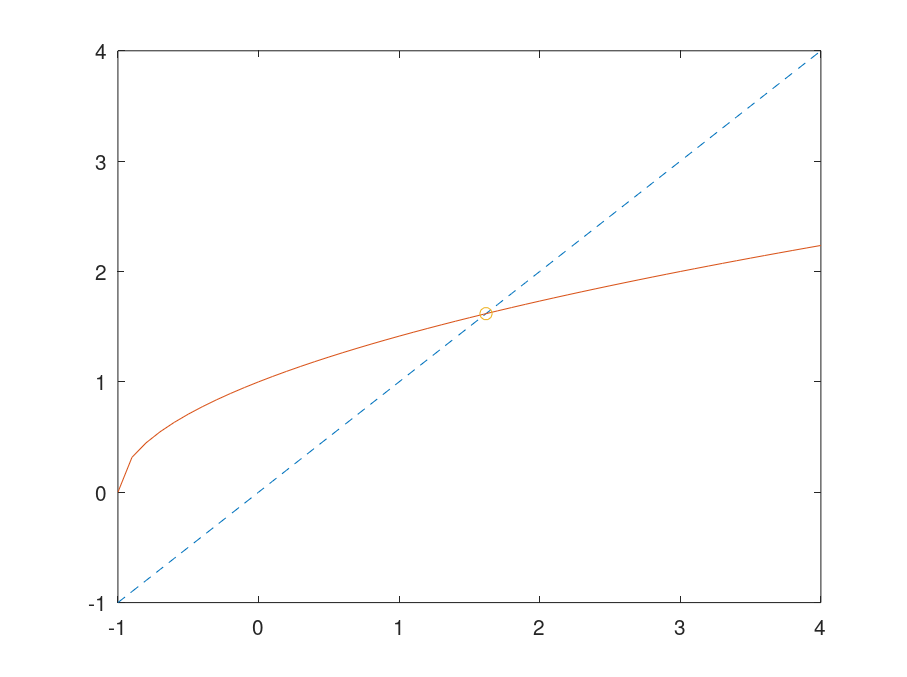
\includegraphics[width=0.5\textwidth]{goldengraph}
	\caption{Numărul de aur}
	\label{fig:1}
\end{figure}

\subsubsection{Puncte fixe}

\textbf{Definiție.} Fie $f: M \rightarrow M$ o funcție continuă și un spațiu
metric $(M, d)$. $f$ este o contracție dacă există un număr real $k \in [0, 1)$
astfel încât
\begin{equation*}
	d(f(x), f(y)) \leq k d(x, y), \quad \forall x, y \in M
\end{equation*}

Cel mai mic număr $k$ pentru care această relație este adevărată se numește
\textit{constantă Lipschitz}. Pentru că $k < 1$, putem spune despre $f$ că este
continuă.

\textbf{Teorema lui Banach.} Dacă $f: M \rightarrow M$ este o contracție pe un
spațiu metric complet $(M, d)$, atunci există un unic punct fix $x^* \in M$
pentru care $f(x^*) = x^*$.

Pe $\mathbb{R}$, distanța o putem considera ca fiind $d(x, y) = |x - y|$.
\begin{align*}
	|f(x) - f(y)|                 & \leq k |x - y| \\
	\frac{|f(x) - f(y)|}{|x - y|} & \leq k         \\
	|\frac{f(x) - f(y)}{x - y}|   & \leq k         \\
\end{align*}
dar, din teorema lui Lagrange, știm că există un $c \in (a, b)$ astfel încât
\begin{equation*}
	|f'(c)| \leq k
\end{equation*}

Astfel, putem spune că iterația $x^{(k+1)} = f(x^{(k)})$ converge către un
punct fix $x^*$ dacă $|f'(c)| < 1$, pentru orice $c \in (a, b)$.

\textbf{Exemplu.} Fie $f(x) = \sqrt{1 + x}$. Calculăm derivata funcției:
\begin{align*}
	f'(x) & = \frac{1}{2} (1 + x)^{-\frac{1}{2}} \\
	f'(x) & = \frac{1}{2 \sqrt{1 + x}}
\end{align*}

Pentru orice $x \in \mathbb{R}, \quad x \geq 0$, avem $|f'(x)| < 1$, deci
funcția este o contracție pe $\mathbb{R}_+$ și are un punct fix unic.

\subsection{Metode iterative pentru sisteme de ecuații liniare}

Folosind teorema de mai sus, putem spune despre transformarea liniară
$T : \mathbb{R}^n \rightarrow \mathbb{R}^n$ că este o contracție dacă
"derivata" transformării este mai mică decât 1. Pentru că $T$ este o funcție
vectorială, derivata se calculează folosind \textit{matricea Jacobiană}. Ne
dorim ca această matrice să aibe norma subunitară, lucru care se întâmplă dacă
matricea are raza spectrală mai mică decât 1.

Considerăm sistemul $Ax = b$. Ne dorim să îl rescriem pentru a ajunge la forma
$x = T(x)$. Metoda prin care vom face asta e să descompunem matricea $A$ în
$A = M - N$.
\begin{align*}
	(M - N)x & = b                  \\
	Mx       & = Nx + b             \\
	x        & = M^{-1}Nx + M^{-1}b
\end{align*}

Astfel, $T(x) = M^{-1}Nx + M^{-1}b$. Notăm $G = M^{-1}N$ și $c = M^{-1}b$. $G$
este \textit{matricea de iterație}, iar $c$ este \textit{vectorul de iterație}.
Jacobiana lui $T$ este chiar matricea $G$, ceea ce înseamnă că, pentru
convergență, avem nevoie ca raza spectrală a lui $G$ să fie mai mică decât 1.
Acest lucru se poate vedea și din analiza erorii:
\begin{gather*}
	x - x^{(k)} = (Gx + c) - (Gx^{(k - 1)} + c) = G(x - x^{(k - 1)}) \\
	e^{(k)} = G^k e^{(0)}
\end{gather*}

Pentru convergență, avem nevoie ca $\lim_{k \to \infty} e^{(k)} = 0 \equiv \lim_{k \to \infty} G^k = 0$.
Pentru o demonstrație mai amplă, se poate consulta \cite{Hansen}.

Pentru alegerea lui $M$ și $N$, vom partiționa matricea $A$ punând în
evidență o matrice diagonală $D$, o matrice strict triunghiular
inferioară $L$ și o matrice strict triunghiular superioară $U$:
\begin{equation*}
	A = D - L - U
\end{equation*}

\begin{center}
	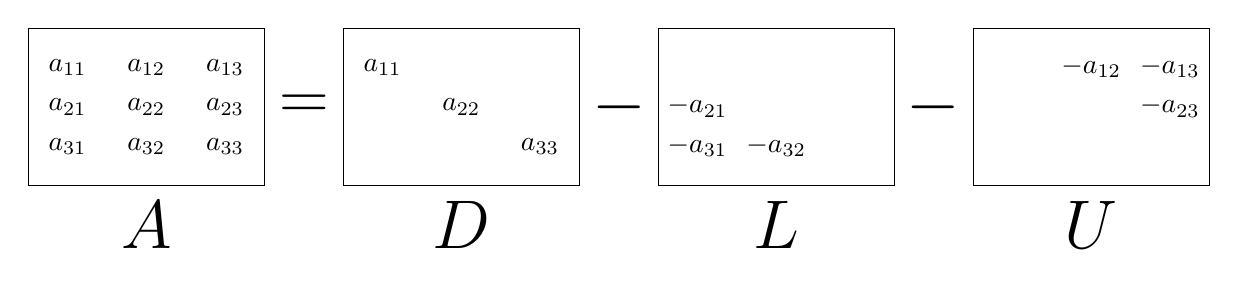
\begin{tikzpicture}
		% Matrix A
		\draw (-2,1) -- (1,1) -- (1,-1) -- (-2,-1) -- cycle;
		\node at (-1.5, 0.5) {$a_{11}$};
		\node at (-0.5, 0.5) {$a_{12}$};
		\node at (0.5, 0.5) {$a_{13}$};
		\node at (-1.5, 0) {$a_{21}$};
		\node at (-0.5, 0) {$a_{22}$};
		\node at (0.5, 0) {$a_{23}$};
		\node at (-1.5, -0.5) {$a_{31}$};
		\node at (-0.5, -0.5) {$a_{32}$};
		\node at (0.5, -0.5) {$a_{33}$};
		\node at (-0.5, -1.5) {\Huge $A$};


		% Arrow to decomposition
		% \draw[thick, ->] (1.5,0) -- (2.5,0);
		\node at (1.5, 0) {\Huge $=$};

		% D matrix
		\draw (2,1) -- (5,1) -- (5,-1) -- (2,-1) -- cycle;
		\node at (2.5, 0.5) {$a_{11}$};
		\node at (3.5, 0) {$a_{22}$};
		\node at (4.5, -0.5) {$a_{33}$};
		\node at (3.5, -1.5) {\Huge $D$};

		% L matrix
		\node at (5.5,0) {\Huge $-$};
		\draw (6,1) -- (9,1) -- (9,-1) -- (6,-1) -- cycle;
		\node at (6.5, 0) {$-a_{21}$};
		\node at (6.5, -0.5) {$-a_{31}$};
		\node at (7.5, -0.5) {$-a_{32}$};
		\node at (7.5, -1.5) {\Huge $L$};

		% U matrix
		\node at (9.5,0) {\Huge $-$};
		\draw (10,1) -- (13,1) -- (13,-1) -- (10,-1) -- cycle;
		\node at (11.5, 0.5) {$-a_{12}$};
		\node at (12.5, 0.5) {$-a_{13}$};
		\node at (12.5, 0) {$-a_{23}$};
		\node at (11.5, -1.5) {\Huge $U$};
	\end{tikzpicture}
\end{center}

Diferența dintre următoarele metode constă în modul în care se asociază aceste
matrice.

% \subsubsection{Metoda bisecției}

% Este o metodă iterativă pentru găsirea rădăcinilor unei funcții continue $f(x)$
% pe un interval $[a, b]$ astfel încât $f(a) \cdot f(b) < 0$. Metoda constă în
% divizarea intervalului în două părți egale și alegerea părții în care se află
% rădăcina (căutare binară).

% Calculăm $c = \frac{a + b}{2}$ și verificăm dacă $|f(c)| < \varepsilon$. Dacă nu,
% în funcție de semnul lui $f(c)$, alegem un nou interval $[a, c]$ sau $[c, b]$.
% Eroare se înjumătățește la fiecare pas și deci
% \begin{align*}
% 	|x^{(k)} - x^*|                   & \leq \frac{b - a}{2^k} \\
% 	\log_2(\frac{b - a}{\varepsilon}) & \leq k
% \end{align*}

% Deci ne trebuie cel puțin $\log_2(\frac{b - a}{\varepsilon})$ iterații pentru a
% obține o precizie de $\varepsilon$.

% Metodele iterative transform\u{a}  sistemul $Ax = b$  \^{i}n $x = Gx + c$. Pornindu-se cu o aproxima\c{t}ie ini\c{t}ial\u{a} ${x}^{(0)}$ a solu\c{t}iei, rela\c{t}ia de recuren\c{t}\u{a}  folosit\u{a} are forma:
% $${x}^{(p+1)} = G{x}^{(p)} + c$$
% unde:
% \begin{itemize}
% 	\item ${x}^{(0)}, {x}^{(1)}, ... , {x}^{(p)}, ...$ sunt aproxim\u{a}rile solu\c{t}iei;
% 	\item $G$ reprezint\u{a} matricea de itera\c{t}ie;
% 	\item $c$ reprezint\u{a} vectorul de itera\c{t}ie.
% \end{itemize}

% \par O metod\u{a} este convergent\u{a} dac\u{a} este stabil\u{a} \c{s}i consistent\u{a}. Condi\c{t}ia necesar\u{a} \c{s}i suficient\u{a} de convergen\c{t}\u{a} este:
% $${\rho}(G) < 1$$
% unde ${\rho}(G) = \max(|{\lambda}_{1}|, |{\lambda}_{2}|, ... , |{\lambda}_{n}|)$ reprezint\u{a} raza spectral\u{a} a matricei de itera\c{t}ie $G$ \c{s}i ${\lambda}_{i}, i = 1:n$ reprezint\u{a} valorile proprii ale matricei.

% \par Metodele iterative se bazeaz\u{a} pe descompunerea matricei $A$ sub forma $A = N - P$. Atunci sistemul devine:

% $(N - P)x = b, $ adică $x = {N}^{-1}Px + {N}^{-1}b.$

% Astfel, rezult\u{a} rela\c{t}ia de recuren\c{t}\u{a}:
% $${x}^{(p+1)} = {N}^{-1}P{x}^{(p)} + {N}^{-1}b$$
% de unde putem identifica $G = {N}^{-1}P$ \c{s}i $c = {N}^{-1}b$.

% \par Se parti\c{t}ioneaz\u{a} matricea $A$ pun\^{a}nd \^{i}n eviden\c{t}\u{a} o matrice diagonal\u{a} $D$, o matrice strict triunghiular inferioar\u{a} $L$ \c{s}i o matrice strict triunghiular superioar\u{a} $U$:
% $$A = D - L - U.$$

\textbf{Condiția de oprire.}  Pentru a finaliza execuția metodelor iterative din
cadrul acestui laborator vom introduce doua condiții: \textbf{toleranța} (notată
în continuare cu \(\epsilon\)) și \textbf{numărul maxim de iterații} (notat în
continuare cu \(N_{iter}\)). Toleranța ne asigură faptul ca algoritmul nu
efectuează iterații mai mult decât este necesar, practic nu se continuă execuția
dacă "diferența" soluțiilor a două iterații consecutive nu este semnificativă.
Numărul maxim de pași garantează că algoritmul se încheie, indiferent dacă
alegerea inițială pentru \(x^{(0)}\) a fost una bună sau nu.

\subsubsection{Metoda Jacobi}
În metoda Jacobi se aleg:
\begin{gather*}
	M = D \\
	N = L + U \\
	G = D^{-1}(L + U) \\
	c = D^{-1}b
\end{gather*}

Pentru că $M$ este o matrice diagonală, inversa sa este foarte ușor de calculat.
Pasul de itarație este:
\begin{align*}
	x^{(k + 1)} & = D^{-1}[(L + U)x^{(k)} + b]                            \\
	x_i^{(p+1)} & = \frac{b_i - \sum_{j \neq i} a_{ij} x_j^{(p)}}{a_{ii}}
\end{align*}

Algoritmul în MATLAB poate fi gândit în două moduri. Cel mai simplu este să
folosim prima relație de mai sus.

\begin{algorithm}
	\caption{Metoda Jacobi}
	\begin{algorithmic}[1]
		\State \( D \gets \text{diag}(\text{diag}(A)) \) \Comment{Extragem Matricea diagonală}
		\State \( L \gets -\text{tril}(A, -1) \) \Comment{Extragem matricea inferior triunghiulară}
		\State \( U \gets -\text{triu}(A, 1) \) \Comment{Extragem matricea superior triunghiulară}

		\State \( G \gets D^{-1} (L + U) \) \Comment{Matricea de iterație}
		\State \( c \gets D^{-1} b \) \Comment{Vectorul de iterație}

		\State \( x \gets \text{zeros}(\text{length}(b),1) \) \Comment{Inițializăm vectorul soluție}
		\State \( i \gets 1 \)

		\While{$i \leq \text{max\_iter}$}
		\State \( x_{\text{prev}} \gets x \)
		\State \( x \gets G \cdot x + c \)
		\If{$\| x - x_{\text{prev}} \| < \text{tol}$}
		\State \textbf{break}
		\EndIf
		\State \( i \gets i + 1 \)
		\EndWhile
	\end{algorithmic}
\end{algorithm}

\subsubsection{Metoda Gauss-Seidel}

În metoda Gauss-Seidel se aleg:
\begin{gather*}
	M = D - L \\
	N = U \\
	G = (D - L)^{-1} U \\
	c = (D - L)^{-1} b
\end{gather*}

În acest caz, matricea $M$ este o matrice inferior triunghiulară, iar inversa
nu mai este așa ușor de calculat. Pasul de iterație este:
\begin{align*}
	x^{(k + 1)} & = (D - L)^{-1}(Ux^{(k)} + b)                                                                         \\
	x_i^{(p+1)} & = \frac{b_i - \sum_{j = 1}^{i-1} a_{ij} x_j^{(p+1)} - \sum_{j = i + 1}^{n} a_{ij} x_j^{(p)}}{a_{ii}} \\
	x_i         & = \frac{b_i - \sum_{j \neq i}^{} a_{ij} x_j}{a_{ii}}
\end{align*}

Diferența dintre metoda Jacobi și Gauss-Seidel constă în faptul că în metoda
Gauss-Seidel, la calculul lui $x_i^{(p+1)}$ se folosesc valorile deja calculate
pentru $x_j^{(p+1)}$ cu $j < i$.


\begin{algorithm}
	\caption{Metoda Gauss-Seidel}
	\begin{algorithmic}[1]
		\State \( x \gets \text{zeros}(\text{length}(b),1) \) \Comment{Inițializăm vectorul soluție}

		\For{$i = 1$ to $\text{max\_iter}$}
		\State \( x_{\text{prev}} \gets x \)
		\For{$j = 1$ to $\text{length}(x)$}
		\State \( x[j] \gets \frac{b[j] - \sum_{k \neq j}^{} A[j,k] x[k]}{A[j,j]} \)
		\EndFor
		\If{$\| x - x_{\text{prev}} \| < \text{tol}$}
		\State \textbf{break}
		\EndIf
		\EndFor
	\end{algorithmic}
\end{algorithm}

De observat la metodele Jacobi și Gauss-Seidel este că o condiție suficientă dar
nu necesară pentru convergența acestora este ca matricea $A$ să fie diagonal
dominantă. Metodele Jacobi și Gauss-Seidel au proprietatea că ori sunt ambele
convergente, ori niciuna nu este convergentă (teorema Stein-Rosenberg). Atunci
când converg, Gauss-Seidel converge mai rapid decât Jacobi, $\rho(GS) < \rho(J) < 1$.

\subsubsection{Metoda suprarelaxării}

O variantă a metodei Gauss-Seidel este metoda suprarelaxării succesive (SOR).
Se introduce un parametru de relaxare $\omega$ și se obține:
\begin{align*}
	A & = M - N                           \\
	A & = M - \omega M - N + \omega M     \\
	A & = (1 - \omega) M - (N - \omega M) \\
	A & = M(\omega) - N(\omega)
\end{align*}

Dacă notăm cu $GS$ formula pentru $x_i^{(p+1)}$ de la Gauss-Seidel, atunci
formula pentru SOR este:
\begin{equation*}
	x_i^{(p+1)} = (1 - \omega) x_i^{(p)} + \omega GS
\end{equation*}

Dacă $A$ este simetrică și pozitiv definită, atunci pentru $\omega \in (0, 2)$
metoda SOR converge. Pentru $\omega = 1$ obținem metoda Gauss-Seidel.

\newpage
\begin{algorithm}
	\caption{Metoda SOR}
	\begin{algorithmic}[1]
		\State \( x \gets \text{zeros}(\text{length}(b),1) \) \Comment{Inițializăm vectorul soluție}

		\For{$i = 1$ to $\text{max\_iter}$}
		\State \( x_{\text{prev}} \gets x \)
		\For{$j = 1$ to $\text{length}(x)$}
		\State \( x[j] \gets \frac{b[j] - \sum_{k \neq j}^{} A[j,k] x[k]}{A[j,j]} \)
		\EndFor
		\State \( x \gets \omega \cdot x + (1 - \omega) \cdot x_{\text{prev}} \) \Comment{Aplicăm relaxarea}
		\If{$\| x - x_{\text{prev}} \| < \text{tol}$}
		\State \textbf{break}
		\EndIf
		\EndFor
	\end{algorithmic}
\end{algorithm}

\section{Probleme}

\begin{questions}
	\question Să se implementeze în MATLAB funcțiile pentru metodele iterative
	Jacobi, Gauss-Seidel și SOR.

	\question Desenați grafic, pentru fiecare metodă, evoluția erorii în funcție
	de numărul de iterații. Testați parametrii diferiți pentru $\omega$ în
	metoda SOR.

	\question Folosiți metoda Jacobi pentru a aproxima soluția sistemului:
	\begin{align*}
		10x_1 - 5x_2 + x_3  & = 1 \\
		x_1 + 4x_2 + 3 x_3  & = 4 \\
		4x_1 - 3 x_2 - 9x_3 & = 6
	\end{align*}

	\question Fie sistemul liniar:
	\begin{align*}
		2x + y + z & = 4 \\
		x + 2y + z & = 4 \\
		x + y + 2z & = 4
	\end{align*}
	Stabiliți convergența metodelor Jacobi și Gauss-Seidel și razele spectrale
	corespunzătoare. În caz de convergență, calculați soluția iterativă după
	trei pași. Alegeți voi aproximația inițială.

\end{questions}

\bibliographystyle{plain}
\bibliography{refs}

\end{document}
